\documentclass[tikz, border=10pt]{standalone}
\usetikzlibrary{calc, automata, chains, arrows.meta, quotes}
\begin{document}
\tikzset{every loop/.style={min distance=10mm,in=120, out=60, looseness=10}}
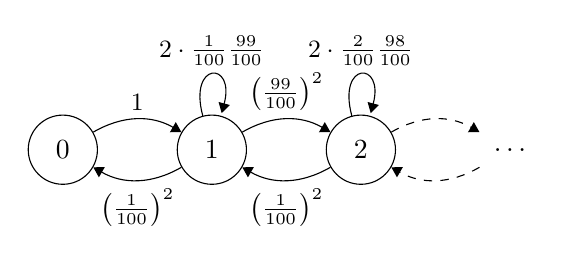
\begin{tikzpicture}[start chain = going right,
  -Triangle, every loop/.append style = {-Triangle}]
\node[state] (A) {$0$};
\node[state] (B) [right = of A] {$1$};
\node[state] (C) [right = of B] {$2$};
\node[state] (E) [right = of C, draw=none]  {$$}; % invisible node
\begin{small}
\draw (A) edge[bend left] node[above] {$1$} (B);
\draw (B) edge[bend left] node[below] {$\left(\frac{1}{100}\right)^2$} (A);
\draw (B) edge[bend left] node[above] {$\left(\frac{99}{100}\right)^2$} (C);
\draw (C) edge[bend left] node[below] {$\left(\frac{1}{100}\right)^2$} (B);
\draw (B) edge[loop above] node[above] {$2\cdot\frac{1}{100}\frac{99}{100}$} (B);
\draw (C) edge[loop above] node[above] {$2\cdot\frac{2}{100}\frac{98}{100}$} (C);
\end{small}
% \node[state] (D) [right = 2cm of C] {$3$};
 \node[state] (D) [right = of C, draw=none] {$\ldots$}; % invisible node
\draw (C) edge[bend left, dashed] (D);
\draw (D) edge[bend left, dashed] (C);
                                % just for arrow
\end{tikzpicture}
\end{document}
